\section{Dokumentasjon}
\subsection{P \& ID} 

Vi tegner P \& ID etter ISO 15519-2 Standaren. Det brukes mange standrer
for P\&ID, men denne er ny og oppdatert. Når en møter på eldre standarder
må en tolke så godt en kan og kanskje finne en beskrivelse i en gammel
norm o.l...

ISO 15519 henter symboler fra ISO 14617 serien. 

ISO 15519-1:2010 Specification for diagrams for process industry \textemdash{}
Part 1: General rules

ISO 15519-2:2015 Specifications for diagrams for process industry
\textemdash{} Part 2: Measurement and control

Kjemisk industri og petroliumsindustien har sin egen standard, som
bygger på ISO 15519, ISO 10628-1 (Diagrams for the chemical and petrochemical
industry. 
Frem til nå har vi sett på flere typer instrument skjema, i alle har de for skjellige instrumentene hatt en kode som forklarer funksjonen. TT er en Termperatur Transmitter, PDT er en Trykk Differanse Transmitter eller FV er en Flow Ventil. Disse bokstavene er definert i ISO 14617-6. 

\vskip 5pt 

\vskip 5pt 

\vskip 5pt 


\vskip 5pt 

% No blank lines allowed between lines of an \halign structure!
% I use comments (%) instead, so that TeX doesn't choke.
\hrule
\small
\begin{center}
\begin{tabular}{ | m{1cm} | m{2.5cm}| m{2cm} | m{2.5cm} |} 
\hline
\multicolumn{4}{|c|}{Bokstavkode for indentifisering av instrumentfunksjoner} \\
\hline
	Bokst. & Variabel& Omformer & Funksjon \\ 
\hline
	A&&&Alarm\\
\hline
	B&&&Visning av diskre status\\
\hline
	C&&&Regulerende\\
\hline
	D&Densitet&Differanse&\\
\hline
	E&Elektrisk variabel&&Elemens (følende)\\
\hline
	F&Flow rate&Forhold&\\
\hline
	G&Posisjon, lengde&&Visning\\
\hline
	H&Håndbetjent&&\\
	\hline
	I&&&Indikerende\\
	\hline
	J&Effekt&Avsøke&\\
	\hline
	K&Tid&Forandring i tid&\\
	\hline
	L&Nivå&&\\
	\hline
	M&Fuktighet eller Relativ fuktighet&&\\
	\hline
	N&Etter brukers valg&&\\
	\hline
	N&Etter brukers valg&&\\
	\hline
	P&Trykk eller vakum&&Tilkobling til testpunkt\\
	\hline
	Q&\makecell{Egenskap\\f.eks:\\*Analyse\\*Konsentrasjon}&Integrere eller summere&Integrerende eller summerende\\
	\hline
	R&Radioaktiv stråling&&Skrivende\\
	\hline
	S&Hastighet&&Bryterfunksjon\\
	\hline
	T&Temperatur&&Overføring\\
	\hline
	U&Multivariabel&&Multifunksjon\\
	\hline
	V&Etter brukers valg& &Påvirkning på prosess med ventil eller pumpe, o.l.\\
	\hline
	W&Vekt, Kraft&Multipliserende&\\
	\hline
	X&Uspesifiserte variabler&&Uspesifisert\\
	\hline
	Y&Etter brukers valg&&Konvertering eller algoritme\\
	\hline
	Z&Antall hendelser, antall&&Nødbetjening eller sikkerhetsfunksjon\\
\hline
\end{tabular}
\end{center}
\normalsize
%Måleteknikk 
\vskip 5pt
\hrule

\vskip 5pt

\subsection{Tegneregler}

\subsubsection{Linjetykkelser}
\begin{itemize}
\item 1.0 mm skal brukes for hovedprosesslinjer
\item 0.5 mm skal brukes på:
\begin{itemize}
\item symboler som representerer makineri, unntatt ventiler og fittings
\item rektangulære rammer som representerer enhetsoperasoner, prosessutstyr,
o.l.
\item Tilleggs prosesslinjer
\item energiforsyningslinjer.
\end{itemize}
\item 0.25 mm skal brukes på.
\begin{itemize}
\item symboler som representerer ventiler, fitting og rørtilbehør.
\end{itemize}
\end{itemize}

\subsection{Informasjonsflyt mellom kontrollsystemet og prosessen. }

\includegraphics[width=1\textwidth]{./PandID01.eps}

\subsection{Plassering av informasjon rundt PCI symboler. }

%\includegraphics[width=0.5\textwidth]{P&ID04}
\subsubsection{Inn og ut av skjemaer}

Linjer som skal fortsette i andre skjemaer skal ha en PIL

%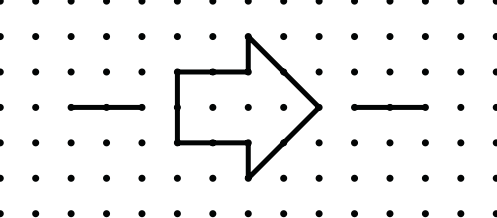
\includegraphics{P&ID05}

Pil for inn- og utgående flow

%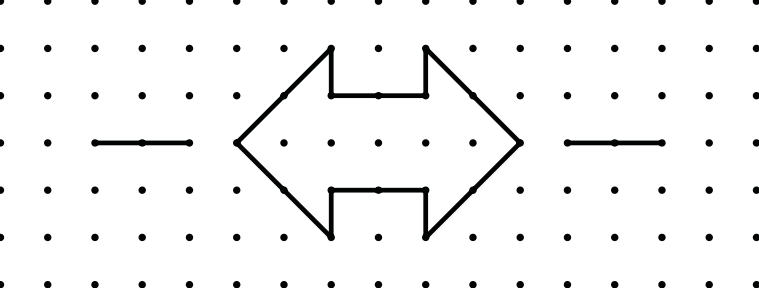
\includegraphics{P&ID06}


\subsection{Referansebetegnelsessystem}
\small
\begin{center}
\begin{tabular}{ | m{1cm} | m{2.5cm}| m{2cm} | m{2.5cm} |} 
\hline
\multicolumn{4}{|c|}{Bokstavkode for utstyri} \\
\hline
	Bokst. & Variabel& Omformer & Funksjon \\ 
\hline
	A&&&Alarm\\
\hline
	B&Sensorer&&Visning av diskre status\\
\hline
	C&Lagring&&Regulerende\\
\hline
	E&Strålende objekt&&\\
\hline
	F&Beskyttende objekt&&\\
\hline
	G&Beskyttende objekt&&\\
\hline
	H&Prossesring av materie&&\\
	\hline
	K&Prosessring av informasjon&&\\
	\hline
	L&Nivå&&\\
	\hline
	M&Objekt som driver noe&&\\
	\hline
	N&&&\\
	\hline
	P&objekt som presenterer&&\\
	\hline
	Q&objekt som presenterer&&\\
	\hline
	R&Objekt som begrenser&&\\
	\hline
	S&Objekt for betjening &&\\
	\hline
	T&Transformerende objekt&&\\
	\hline
	U&Objekt som holder&&\\
	\hline
	W&Førende objekt&&\\
	\hline
	X&Objekt for overgang&&\\
	\hline
\hline
\end{tabular}
\end{center}
\normalsize
%Måleteknikk 
\vfil \eject
\subsection{Symboler}
\includegraphics[width=1\textwidth]{diagrams00.eps}
\includegraphics[width=1\textwidth]{diagrams01.eps}
\includegraphics[width=1\textwidth]{diagrams03.eps}
\includegraphics[width=1\textwidth]{diagrams13.eps}
\includegraphics[width=1\textwidth]{diagrams05.eps}
\includegraphics[width=1\textwidth]{diagrams02.eps}
%\includegraphics[width=1\textwidth]{diagrams04.eps}
%\includegraphics[width=1\textwidth]{diagrams06.eps}
%\includegraphics[width=1\textwidth]{diagrams07.eps}
%\includegraphics[width=1\textwidth]{diagrams10.eps}
%\includegraphics[width=1\textwidth]{diagrams11.eps}
%\includegraphics[width=1\textwidth]{diagrams12.eps}
%\includegraphics[width=1\textwidth]{diagrams14.eps}
